\section{Versuchsdurchführung}

Der Winkel $\alpha$ wird mithilfe einer Winkelmessung $\beta$ zwischen der schiefen Ebene und der Vertikalen gemessenen. Da die Vertikalen nicht im $90^\circ$ Winkel zu der Horizontalen steht, wird der Winkel $\gamma$ gemessenen. Mit \autoref{eq:alpha} wird $\alpha$ berechnet.

\begin{align}
    \alpha = 90^\circ - (\beta - (90^\circ - \gamma))
    \label{eq:alpha}
\end{align}

\begin{figure}[ht]
    \center
    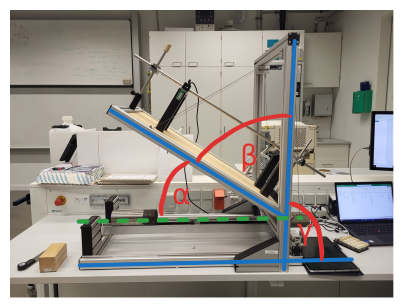
\includegraphics{images/Versuch-Winkel.pdf}
    \caption[Winkelmessung]{Winkel $\alpha$, $\beta$ und $\gamma$}
    \label{fig:Winkelmessung}
\end{figure}